%%%%%%%%%%%%%%%%%%%%%%%%%%%%%%%%%%%%%%%%%%%%%%%%%%%%%%%%%%%%%%%%%%%%%%%%%%%%%%%
\subsection{Apache Spark and Spark SQL overview}
% \label{sec:}
% \input{}
%%%%%%%%%%%%%%%%%%%%%%%%%%%%%%%%%%%%%%%%%%%%%%%%%%%%%%%%%%%%%%%%%%%%%%%%%%%%%%%
%\mytodo{Intro to spark, refer to spark paper: the paradigm, the abstraction, speed, ...}.
In this paper, we adopt an open-source processing engine: Apache Spark. Among the prevalent engines, Spark is proven to bring strong performance due to its in-memory computation nature. It is the first cluster computing engine that leverages the distributed memory abstraction and outperforms Hadoop by up to 20X in iterative applications \cite{zaharia2012resilient}. This motivated us to propose a new in-memory cache-based optimization for cloud environment. Spark SQL is the high level language support running on top of Spark. We present the implementation of our solution in the query optimizer of Spark SQL.

Spark SQL defines an SQL-like high-level language for processing large-scale analytic workloads. The queries expressed in the high-level languages are finally transformed into RDDs as the abstract concept of Spark core engine. Queries written in Spark SQL are in an abstract form: the DataFrames. A DataFrame object represents a \emph{logical plan} to compute a dataset. A logical plan is a tree composed of operators (nodes). Each has operator name (operator type) and attributes (filtering predicates, join columns, etc.). A node could be binary, unary or leaf node that has 2 children, 1 child or zero child respectively.

Catalyst \cite{sparksql} is the query optimizer of Spark SQL. Catalyst focuses on optimizing each single query, while in our approach, a cost-based optimizer is applied to optimize multiple queries together. The rule-based optimizer in Spark SQL defines the rules (constant folding, early filtering, and predicate pushdown, etc.) to produce optimized logical plans. Using the cost model to decide the joining strategies, the optimized logical plans are then transformed to single physical plan for execution. Figure \ref{fig:sparksql_queryplanning} illustrates the internal Spark SQL's architecture, and the modules involved in parsing and generating the various query plans discussed above.

\begin{figure*}[t]
   \centering
   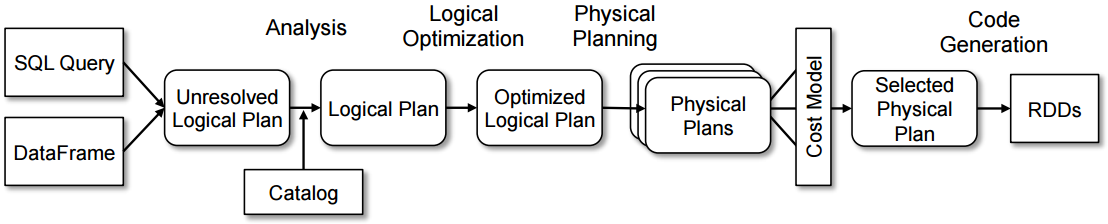
\includegraphics[scale=0.45]{figures/sparksql_queryplanning}
   \caption{Phases of query planning in Spark SQL. Rounded rectangles represent Catalyst trees \cite{sparksql}} 
   \label{fig:sparksql_queryplanning}
\end{figure*}

%%%%%%%%%%%%%%%%%%%%%%%%%%%%%%%%%%%%%%%%%%%%%%%%%%%%%%%%%%%%%%%%%%%%%%%%%%%%%%%
\subsection{Implementation of work sharing for Spark SQL}
\label{sec:plan_implementation}
In Spark SQL, for each individual application, it is possible to indicate which data (DataFrame) to cache in memory. Subsequent data transformation can reuse cached data without the need to recompute it from the lineage. However, Spark applications submitted to a cluster by different clients are totally isolated from each other\cite{zaharia2012resilient}, therefore, sharing across applications is not trivial. To avoid modifying spark's internal architecture principle, we build a centralized Spark SQL server serving requests from multiple users while acting as a single client of cluster. The optimization we proposed is being done at this central Spark SQL server.

In our system, we use the optimized logical plans as the input for the query optimizer. Users have many interfaces to express the data they want in Spark SQL. Logical plan is the one that abstract and unified. The optimized logical plan is the last logical representation of a query before converting it to a physical. If the input queries are similar, looking at the optimized logical plans is the best way to discover the similar parts.

We follow the optimization process of 4 phases discussed in section \ref{sec:caching}. Operator fingerprints are computed to identify all similar subexpressions in the first phase. Phase 2 and phase 4 require some query transformations. We take advantage of the pattern matching feature of scala and the TreeNode library of Catalyst in Spark SQL to rewrite queries. Transforming rules are passed as a function to specify how to transform the trees. Pre-computed statistics data computed in phase 3 are done by launching 2 jobs for each table. The cardinality of each column is estimated using the algorithm HyperLogLog.

